%  $
% \newcommand{\MtdFull}[1]{\frac{D \, #1}{D \, t}}
% \newcommand{\Pd}[2]{\frac{\partial #1}{\partial #2}}
% \newcommand{\d}{\text{d} }
% \newcommand{\Dd}[2]{\frac{\d #1}{\d #2}}
% \newcommand{\dt}[1]{#1 ^{\bullet}}
% \newcommand{\dV}{\; \text{d}V}
% \newcommand{\dA}{\; \text{d}A}
% \newcommand{\dx}{\; \text{ d}x}
% \newcommand{\dy}{\; \text{ d}y}
% \newcommand{\dz}{\; \text{ d}z}
% \newcommand{\dxi}{\; \text{ d}\xi}
% \newcommand{\deta}{\; \text{ d}\eta}
% \newcommand{\dzeta}{\; \text{ d}\zeta}
% \newcommand{\grad}[1]{\text{grad}\left(#1\right)}
% \renewcommand{\div}[1]{\text{div} \left(#1\right)}
% \newcommand{\td}[1]{\dot{#1}}
% \newcommand{\tdd}[1]{\ddot{#1}}
% \newcommand{\T}{\rp{T}}
% \newcommand{\rp}[1]{^{\text{#1}}}
% \newcommand{\rs}[1]{_{\text{#1}}}
% \renewcommand{\bm}[1]{\boldsymbol{#1}}
% \newcommand{\e}{\epsilon}
% \newcommand{\eb}{\bm{\e}}
% \newcommand{\s}{\sigma}
% \newcommand{\sb}{\bm{\sigma}}
% $

\subsubsection{Von der starken zur schwachen Form}

Für die in Kapitel 1 eingeführten Randwertprobleme (Massenbilanz, Impulsbilanz und Energiebilanz) werden in diesem Kapitel die theoretischen Grundlagen der Finite Elemente Methode beschrieben. Für jedes der genannten Probleme ist der Ausgangspunkt die \textbf{starke} Form der beschreibenden partiellen Differentialgleichung. Am Beispiel der Impulsbilanz soll exemplarisch die zugehörige \textbf{schwache} Form hergeleitet werden. Die Begriffe stark und schwach beziehen sich hierbei auf die Stetigkeits- und Differenzierbarkeitsanforderungen der gesuchten Lösung $\bm{u}$. Die starke Form hat somit \textbf{immer} höhere Anforderungen an die Lösung.

\begin{figure}[!htbp]
\centering
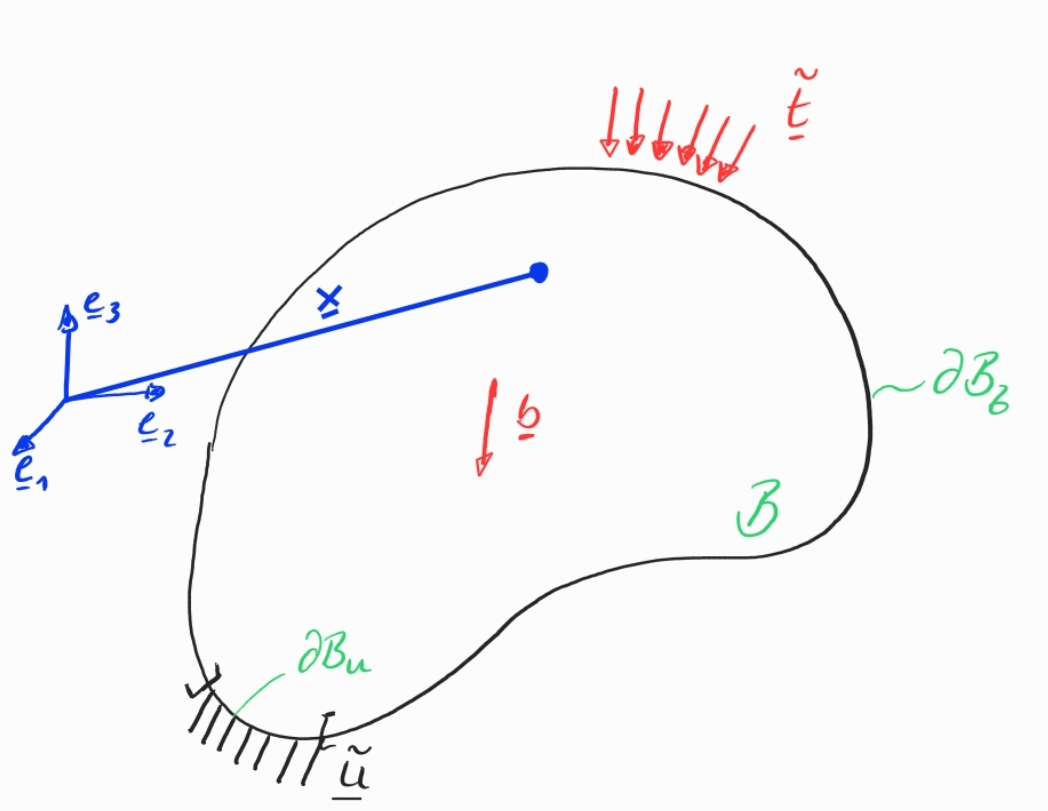
\includegraphics[width=0.7\linewidth]{files/Impulsbilanz-3c1ed32b03eec7db5f7e582ea9b4a7c5.jpg}
\caption[]{Körper $\mathcal{B}$ unter Einwirkung der externen Oberflächenkraft $\tilde{\bm{t}}$ und der Volumenlast $\bm{b}$}
\label{impulsbilanz_fig}
\end{figure}

Ausgangspunkt für die exemplarische Herleitung ist die Impulsbilanz in der quasistatischen Form (ohne Trägheitsterme):

\begin{equation}
\label{weakform_01}
0 = \div{\bm{\sigma}} + \rho \bm{b}
\end{equation}
Diese starke Form wird jetzt mit einer beliebigen vektorwertigen Testfunktion $\delta \bm{u}$ multipliziert und über das betrachtete Gebiet $\mathcal{B}$ (den betrachteten Körper) integriert.

\begin{equation}
\label{weakform_02}
0 = \int_{\mathcal{B}} \delta  \bm{u}\T \left(\div{\bm{\sigma}} + \rho \bm{b} \right) \dV
\end{equation}

Dieser Schritt bedeutet, dass wir im Weiteren versuchen werden, die gekoppelten partiellen Differentialgleichungen nicht punktuell exakt zu erfüllen, sondern im gewichteten integralen Mittel. Für elastomechanische Problemstellungen kann die Testfunktion $\delta \bm{u}$ als virtuelle Verrückung aufgefasst werden, und die Gleichung (\ref{weakform_02}) als das bekannte Prinzip der virtuellen Verrückung angesehen werden. Das hier gezeigte Vorgehen ist jedoch unabhängig von der Elastostatik allgemeingültig.

Als Nächstes integrieren wir die Gleichung (\ref{weakform_02}) partiell. Dafür wenden wir zunächst die Produktregel auf den Divergenzterm an:

\begin{equation}
\label{divergenzsatz}
\int_{\mathcal{B}} \delta \bm{u}\T \div{\bm{\sigma}} \dV = \int_{\mathcal{B}} \div{\delta \bm{u}\T \bm{\sigma}} \dV -\int_{\mathcal{B}} \underbrace{\grad{\delta\bm{u}\T}}_{\delta \bm{\eb}}\bm{\sigma} \dV \; .
\end{equation}

Der Wechsel vom Divergenz-Operator zum Gradienten-Operator im zweiten Term auf der rechten Seite lässt sich schlüssig damit erklären, dass das Resultat ein Skalar sein soll. Während die Divergenz eines Vektors einen Skalar liefert, ergibt der Gradient eines Vektors einen Tensor zweiter Ordnung. Dieser Tensor wird dann in einer doppelten skalaren Multiplikation mit einem weiteren Tensor zweiter Ordnung verknüpft, was letztlich zu einem skalaren Ergebnis führt.

Nun lässt sich mit dem Gau$\beta$'schen Integralsatz der erste Term auf der rechten Seite von Gleichung (\ref{divergenzsatz}) als Integral über den Rand formulieren:

\begin{equation}
\label{gaussIntegralTheorem}
\int_{\mathcal{B}} \div{\delta \bm{u}\T  \bm{\sigma}} \dV = \int_{\partial\mathcal{B}} \delta \bm{u}\T \bm{\sigma}  \bm{n} \dA = \int_{\partial\mathcal{B}} \delta \bm{u}\T \bm{t} \dA \; .
\end{equation}

Dieses Resultat wird jetzt wieder in Gleichung (\ref{weakform_02}) eingesetzt und wir erhalten:

\begin{equation}
\label{weakform_03}
\int_{\mathcal{B}} \delta\eb\T  \bm{\sigma} \dV = \int_{\mathcal{B}} \delta \bm{u}\T \rho \bm{b} \dV + \int_{\partial\mathcal{B}} \delta \bm{u}\T  \bm{t} \dA \; .
\end{equation}

\begin{framed}
\textbf{Was haben wir damit erreicht?}\\
\begin{itemize}
\item Der Oberflächenterm in (\ref{weakform_03}) entspricht den Kraftrandbedingungen
\item Der Term auf der linken Seite in (\ref{weakform_03}) enthält nur noch Ableitungen 1. Ordnung von $\bm{u}$, während in (\ref{weakform_01}) Ableitungen 2. Ordnung gefordert wurden $\rightarrow$ schwächere Anforderungen an $\bm{u}$!
\item Gleichung (\ref{weakform_03}) ist exakt das Prinzip der virtuellen Verrückungen\begin{itemize}
\item Virtuelle Arbeit der Spannungen an den Verzerrungen ist gleich der virtuellen Arbeit der eingeprägten Volumenkräfte plus die virtuelle Arbeit der Oberflächenkräfte
\end{itemize}
\end{itemize}
\end{framed}

Setzen wir jetzt noch als Materialmodell die Beschreibung der linearen Elastizität ein, so erhalten wir final:

\begin{equation}
\label{weakform_04}
\int_{\mathcal{B}} \delta\eb\T \bm{C} \eb \dV = \int_{\mathcal{B}} \delta \bm{u}\T \rho \bm{b} \dV + \int_{\partial\mathcal{B}} \delta \bm{u}\T \cdot \bm{t} \dA \; .
\end{equation}

\begin{framed}
\textbf{Fragen zum Kapitel}\\
\textbf{Finite Elemente Methode}

\begin{itemize}
\item Worauf beziehen sich die Begriffe \textit{starke} und \textit{schwache} Formulierung?
\item Was ist korrekt:\begin{itemize}
\item Bei der schwachen Formulierung wird die Bilanzgleichung nur noch im integralen Mittel gelöst.
\item Das Prinzip der virtuellen Verrückung und die schwache Formulierung der Impulsbilanz sind äquivalent.
\item Die starke Formulierung der Bilanzgleichung enthält Ableitungen höherer Ordnung im Vergleich zur schwachen Formulierung.
\end{itemize}
\end{itemize}
\end{framed}